
\documentclass[11pt]{article}
\usepackage{graphicx}
\usepackage{listings}
\usepackage{multirow}
\usepackage[english]{babel}
% Titre complet
\title{Report}

\author{Anna Liednikova}


\begin{document}


\section{Introduction}

Task description: using existing dataset with labeled intents find word embendings that will allow to expand expand it by external data.

\section{Literature review}

\cite{N18-2058} James Ferguson et al faced a similar problem with a small labelled dataset. In their article they describe the approach of automatically expanding dataset and improving the performance of baseline models, that was event trigger identification system in their case.

First, they trained a baseline classifier on available data. Then they identified clusters of additional data to obtain grouped paraphrases inspired by the NewsSpike idea introduced in Zhang et al. (2015). After they labelled clusters with baseline model trained fully-supervised. Combining new labelled data and original one they retrained the event extractor. (Semi-Supervised Event Extraction with Paraphrase Clusters: http://aclweb.org/anthology/N18-2058)



\section{Project}

\subsection{Preprocessing routine}

Before exploring and making dataset statistics proprocessing routine should be covered.

For preprocessing spacy was used. Sentence tokenization, word tokenization, stop words removing and stemming. Length < 30. Stopwords list - basic from spacy.

\subsection{Datasets}

\subsubsection{Dataset with intents}

The initial dataset is created manually covering 20 main possible users intents. Each sentence represents one intent. For, example,

\begin{lstlisting}
{'text': 'After sleep, for 2-3 hours, 
I am better and then start feeling tired again',
 'intent': 'sleep',
}
\end{lstlisting}

Distribution of labels is show on fig. \ref{figure:name}

 \begin{figure}[h]
 	\centering
 	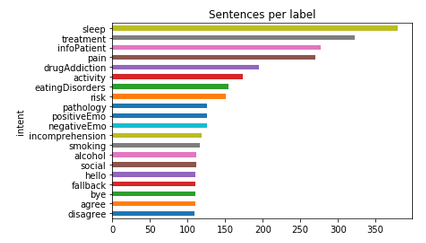
\includegraphics[scale=0.5]{report1.png}
	\caption{Label distribution in dataset}
 \label{figure:name}
 \end{figure}


Total number of sentences is 3307. Found 1880 words after filtering through stopwords list. 

\subsubsection{Forum data}

Thanks to Zhang et al (2015) and Sondhi et al (2010) 

272553 unique posts

{'min': 0, 'max': 2027, 'mean': 10.932588521491454, 'std': 8.964716092053479}
{'min': 3.2580388329566468, 'max': 35.23600634007455, 'mean': 11.224462266261876, 'std': 6.963225985041148}


 \begin{figure}[h]
 	\centering
 	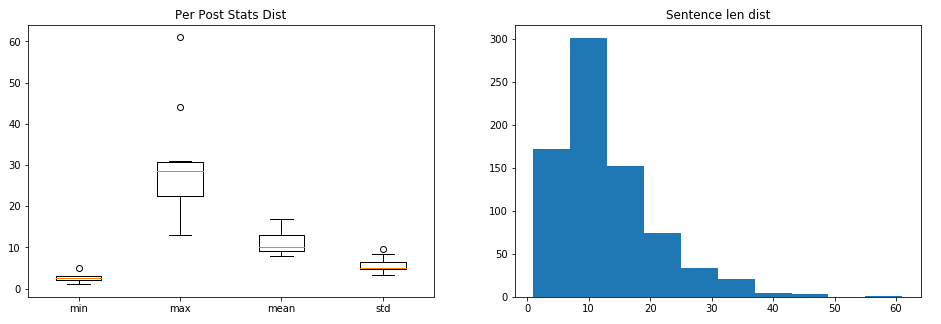
\includegraphics[scale=0.5]{report3.png}
	\caption{Text stat}\label{visina8}
 \end{figure}

Data should be divided in subsets by increasing sentence length because of the difference in mean values for both datasets.


\subsection{Sentence representation models}

From gensim library: LDA (Latent Dirichlet Allocation), Word2Vector model.

Pytorch PositionwiseFeedForward, BiLSTM

\subsubsection{Whole sentence representation}

\subsubsection{Sentence representation by words}

\subsection{Evaluation}

\subsubsection{Clustering models}

Clustering models: 
\begin{itemize}
\item K-Means (KM)
\item AgglomerativeClustering(‘ward’) (AG)
\item GaussianMixture (GM)
\end{itemize}

Number of clusters =  number of intents = 20

Metrics to evaluate: purity, Silhouette Coefficient, homogeneity and completeness.

Describe each model by metrics.



\subsubsection{Classification models}

SVC

\section{Experiment}

\subsection{W2V model}

Comparision table

\begin{tabular}{ |p{2cm}|p{1cm}|c|c|c|c|p{1cm}| }
\hline
WE & Cluster & purity & Silhouette & homogeneity & complete & Clf CV score \\ \hline
\multirow{3}{*}{Defenders} & KM & & & & &\\
 & AC & & & & &\\
 & GM & & & & &\\ \hline
\multirow{3}{*}{M} & KM & & & & &\\
 & AC & & & & &\\
 & GM & & & & &\\ \hline
Forward & FW & & & & &\\ \hline
\multirow{3}{*}{S} & KM & & & & &\\
 & AC & & & & &\\
 & GM & & & & &\\
\hline
\end{tabular}


\subsection{LDA model}


\subsection{GloVe pretrained}

\subsection{Google News W2V pretrained}

\subsection{CNN by word}

\subsection{BiLSTM by word}


\section{Conclusion}

\bibliographystyle{alpha}
\bibliography{report}

\section{References}

@InProceedings{N18-2058,
  author = 	"Ferguson, James
		and Lockard, Colin
		and Weld, Daniel
		and Hajishirzi, Hannaneh",
  title = 	"Semi-Supervised Event Extraction with Paraphrase Clusters",
  booktitle = 	"Proceedings of the 2018 Conference of the North American Chapter of the Association for Computational Linguistics: Human Language Technologies, Volume 2 (Short Papers)",
  year = 	"2018",
  publisher = 	"Association for Computational Linguistics",
  pages = 	"359--364",
  location = 	"New Orleans, Louisiana",
  url = 	"http://aclweb.org/anthology/N18-2058"
}

@InProceedings{sondhi-EtAl:2010:POSTERS,
  author    = {Sondhi, Parikshit  and  Gupta, Manish  and  Zhai, ChengXiang  and  Hockenmaier, Julia},
  title     = {Shallow Information Extraction from Medical Forum Data},
  booktitle = {Coling 2010: Posters},
  month     = {August},
  year      = {2010},
  address   = {Beijing, China},
  publisher = {Coling 2010 Organizing Committee},
  pages     = {1158--1166},
  url       = {http://www.aclweb.org/anthology/C10-2133}
}


@article{article,
author = {Zhang, Thomas and H D Cho, Jason and Zhai, Chengxiang},
year = {2015},
month = {03},
pages = {},
title = {Understanding User Intents in Online Health Forums},
volume = {19},
journal = {IEEE journal of biomedical and health informatics},
doi = {10.1109/JBHI.2015.2416252}

}

\paragraph{APA}

Zhang, T., Cho, J. H. D., \& Zhai, C. (2015). Understanding User Intents in Online Health Forums. IEEE Journal of Biomedical and Health Informatics, 19(4), 1392-1398. [7066225]. https://doi.org/10.1109/JBHI.2015.2416252

\paragraph{Harvard}

Zhang, T, Cho, JHD \& Zhai, C 2015, 'Understanding User Intents in Online Health Forums' IEEE Journal of Biomedical and Health Informatics, vol. 19, no. 4, 7066225, pp. 1392-1398. https://doi.org/10.1109/JBHI.2015.2416252


\end{document}
